\documentclass[conference]{IEEEtran}
\IEEEoverridecommandlockouts
% The preceding line is only needed to identify funding in the first footnote. If that is unneeded, please comment it out.
\usepackage{amsmath,amssymb,amsfonts}
\usepackage{algorithmic}
\usepackage{graphicx}
\usepackage{textcomp}
\usepackage{xcolor}
\bibliographystyle{apalike}


\def\BibTeX{{\rm B\kern-.05em{\sc i\kern-.025em b}\kern-.08em
    T\kern-.1667em\lower.7ex\hbox{E}\kern-.125emX}}
\begin{document}

\title{Style Classification in Posters\\
}

\author{\IEEEauthorblockN{Tim Löhr}
\IEEEauthorblockA{\textit{Friedrich Alexander University} \\
\textit{Pattern Recognition Lab}\\
tim.loehr@fau.de}
}


\maketitle

\begin{abstract}

Digitalization, Big Data and data collection is the keyword of many companies nowadays. Even museums digitize their artworks. A local museum from Bayreuth photographed 17786 posters showing invitations to exhibitions or advertising for specific events. Our department received this data to find patterns in it. More specifically, one shall order the posters in clusters to sort them logically.
Furthermore, if there is a new poster, the clustering should present all posters with similar attributes. Since how to do it was relatively open, I tried four different methods to cluster the posters. First, I used a supervised approach with a neural network and another dataset from WikiArt to perform Transfer Learning. The following two approaches are based on the text printed on the posters. I extracted the text and first performed clustering with the BERT Topic Modeling approach, then with the LDA Topic Modeling approach. Lastly, I focused on the image by extracting the features with a pre-trained neural network and then performing PCA and K-Means to find a pre-defined number of clusters. The three unsupervised approaches produced some output that is workable but is not satisfactory enough.

\end{abstract}
\begin{IEEEkeywords}
neural networks, LDA, BERT, classification, poster, wikiart, museum, clustering
\end{IEEEkeywords}

\section{Introduction}
Data is gathered almost everywhere. For this project, a local museum in Bayreuth took 17786 posters showing different kinds of museum exhibitions. The pictures came in different sizes and with some of them showing only the poster itself, but with some, the background or tables are also visible. The providers of the dataset aim to sort the posters in some way. It shall therefore be researched if the images are sufficient enough to cluster and group them. For this project, I used different techniques to analyze the potential clusters of these images. Figure \ref{fig:poster} illustrates an example poster from the dataset. Some of the problematic properties of the images can already be seen in this picture.

\begin{figure}
\centering
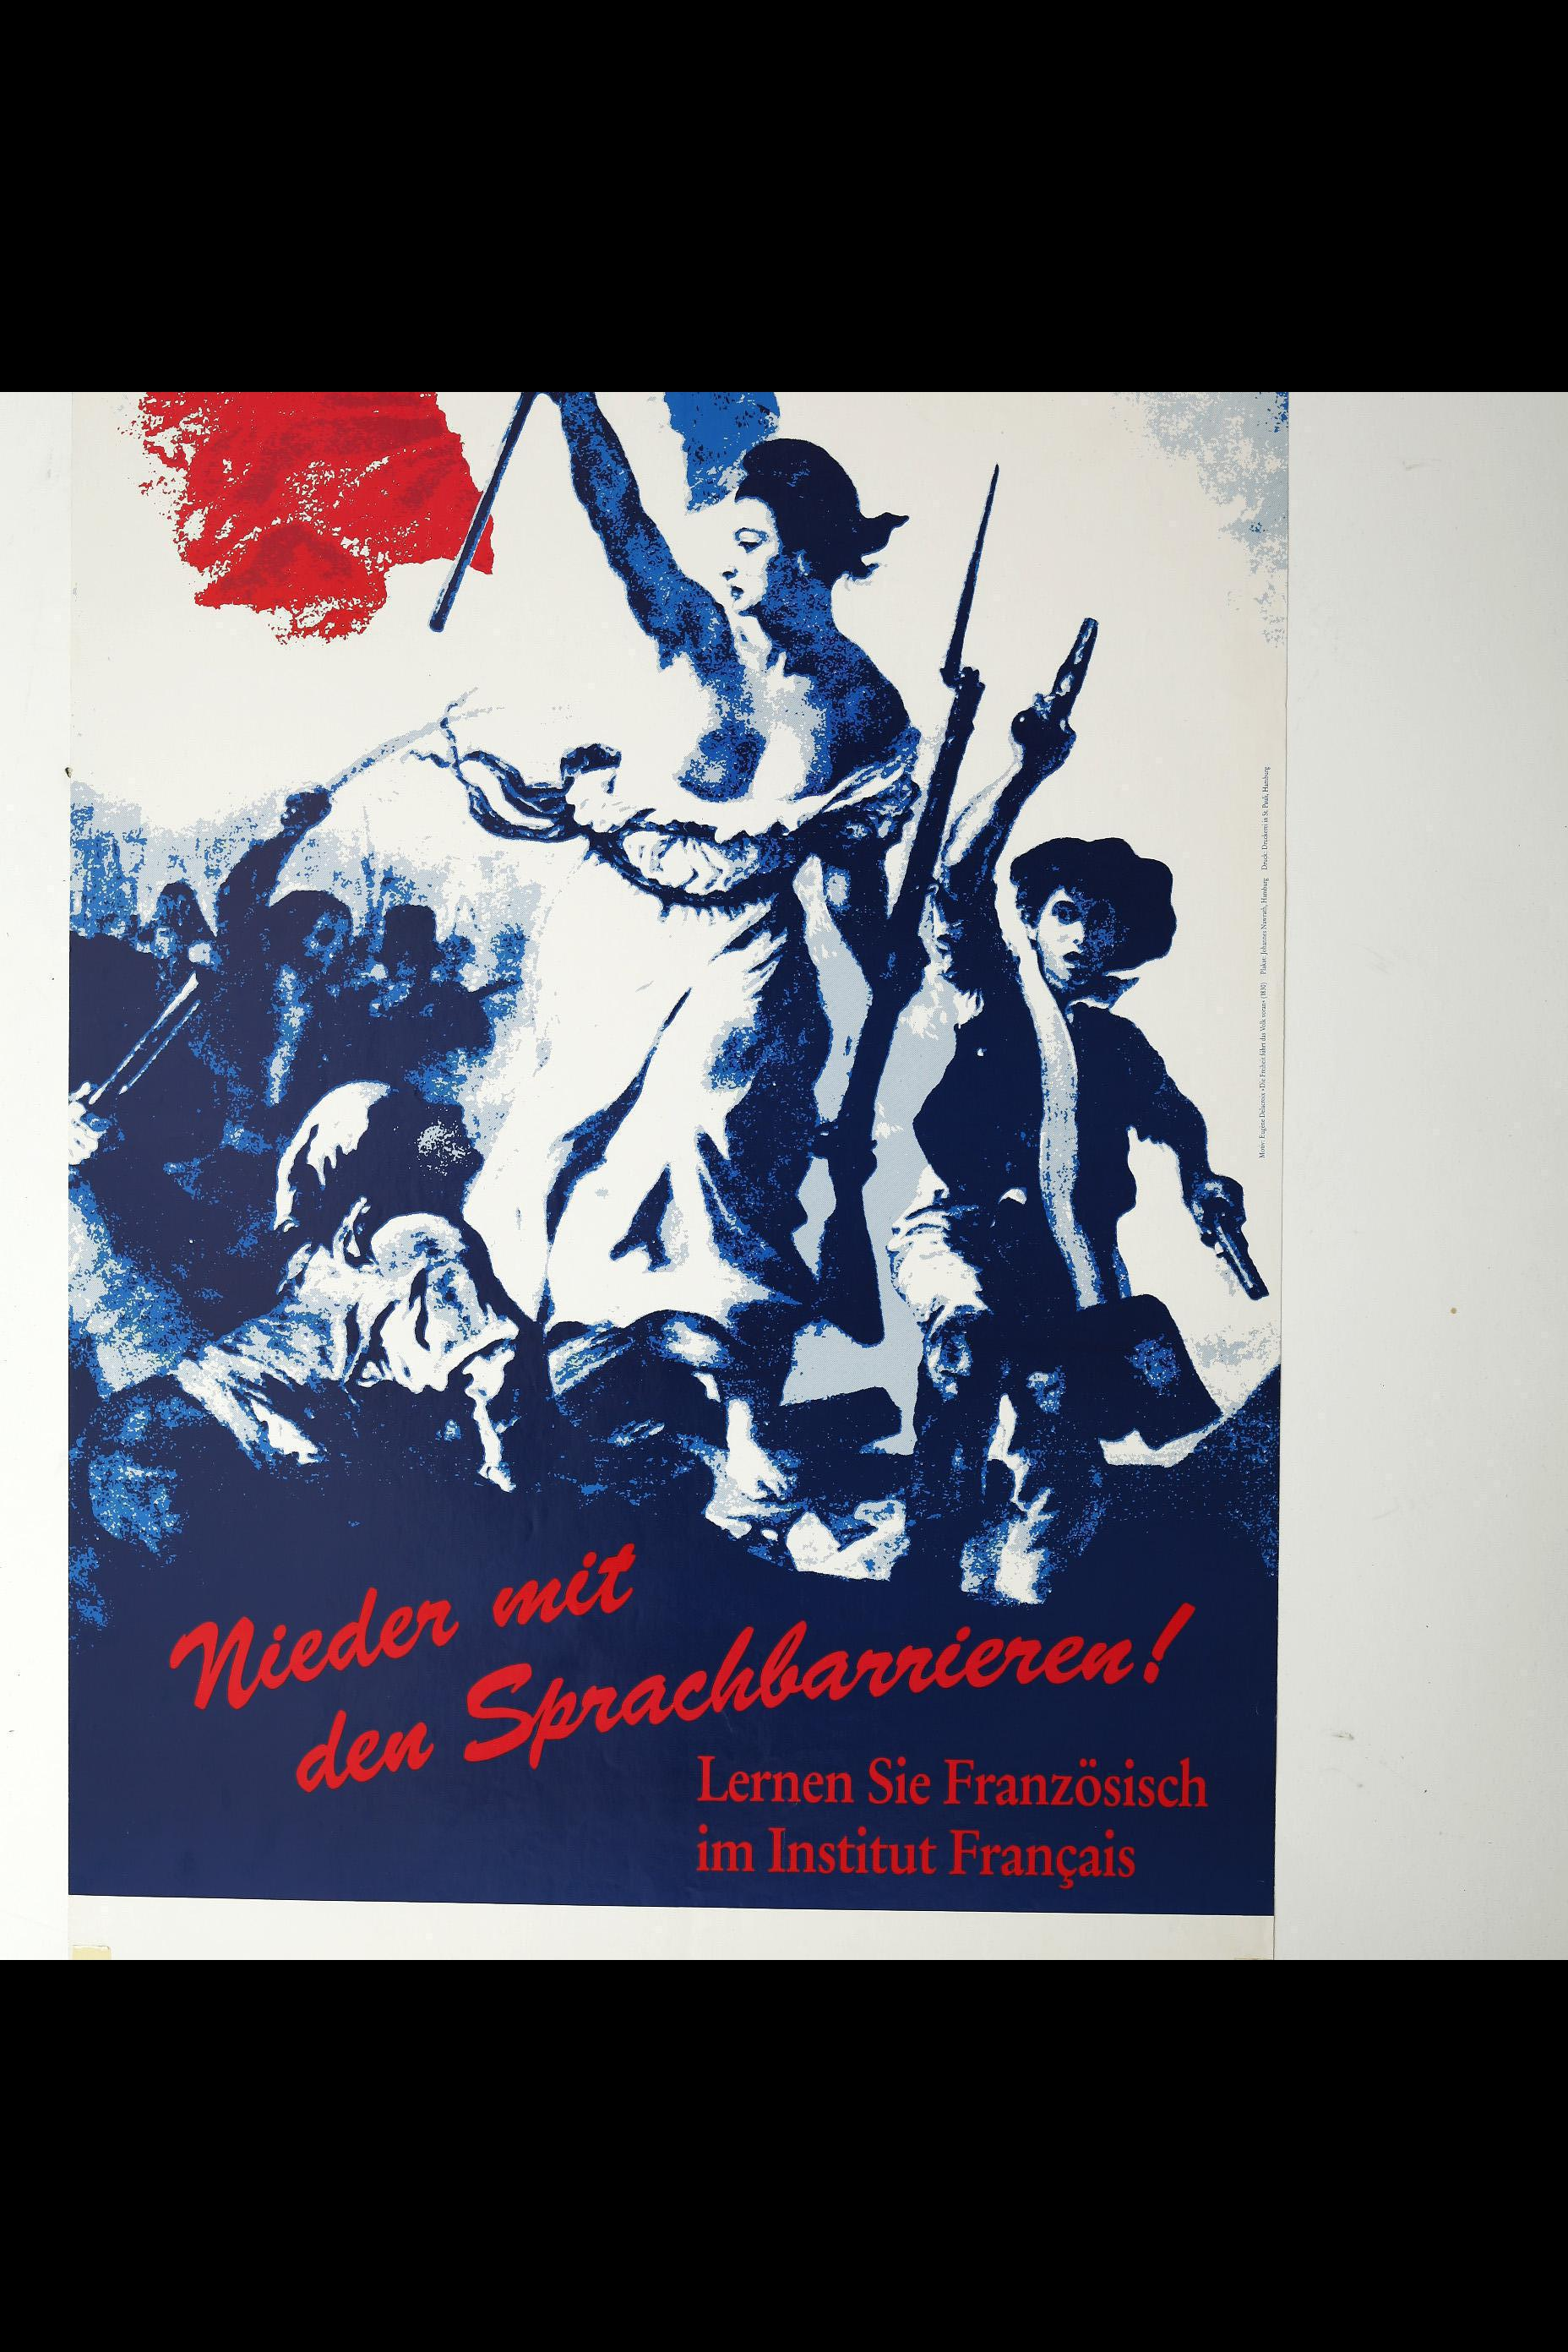
\includegraphics[width=1\linewidth]{../Imgs/acht1_042}
\caption{Sample image from the poster dataset from the Bayreuther museum. It can be seen that we have a white frame on the right side of the image and black frames on the top and at the bottom. Also, both the German and the English language is present as text in the image. Luckily the rotation is correct, but that is only for 25\% of images the case.}
\label{fig:poster}
\end{figure}

\section{Problem Statement}
The thousands of posters come in different shapes and qualities. Not only is this problematic for training a neural network, which requires a fixed-size input, but the posters also come in random rotation. For us as humans, it is easily detectable in which direction the poster has to point to be correct, but not for the neural network. Furthermore, the images amount to a total of 7 Gigabytes, and this requires a lot of computing power to train neural networks or other kinds of machine learning algorithms. This project aims to find clusters within these posters to somehow search through the 17786 pictures or possibly find similar posters given a new poster. At least 50\% of the posters contain more than one word, so a text-based clustering or searching algorithm could be sufficient. Furthermore, some posters like Figure \ref{fig:poster} are designed in a specific style, so maybe transfer learning and classification could do the trick. Therefore, I want to find out if the poster images can be ordered somehow, but the approach needs to be evaluated and tested. 

The research question for this project can therefore be concluded into \\

\textit{Is it possible to cluster the posters and find similar posters given a new image?}

\section{Methods}
Since the research question binds not to a particular approach, I used four different approaches to find similar posters given a poster. The first method aimed to perform classification with Transfer Learning; the other three approaches perform unsupervised learning and identify an unknown number of clusters. Since the problem statements point out different pinpoints, different methods need to be tested to find the best working one. Each of these approaches had its pros and cons, but most of them required a lot of computing power. For this project, I used an Nvidia RTX 3080 Ti. 


\subsection{Style Classification}
For this approach, I used data from WikiArt \footnote{www.wikiart.org} to train a Transfer Learning neural network. Since the poster dataset is not labeled, it seems like a good approach to perform Transfer Learning. This technique allows using a trained network from a similar domain to predict the labels it was trained on. A survey of Transfer Learning points out that for my specific problem, this could be a good approach if another dataset from a similar domain is used \cite{Zhuang.07.11.2019}.

Wikiart is an open platform that provides images of famous painters to download. The pictures from WikiArt show the ancient painting, but there is also an extensive description of the year, style, and genre provided. I used the tool from lucasdavid \footnote{https://github.com/lucasdavid/wikiart} to download the data from WikiArt. In total, I downloaded 17.2 Gigabytes of WikiArt images. The idea is that these paintings can infer the style of the posters provided by the museum and therefore implicitly cluster the images based on their predicted style. If the neural network would learn how, e.g., \textit{Expressionism} in a painting looks like, it could identify all posters that advertise for expressionism exhibitions. For the WikiArt images, there exist more than 400 different genres. I selected only the 20 most common genres, because they covered more than 70\% of all the image labels. That was important to have an train dataset with evenly distributed labels.

The WikiArtimages all had different sizes, so I had to use different data augmentation methods like \newline

\begin{itemize}
\item RandomAffine
\item ColorJitter
\item RandomHorizontalFlip
\item RandomVerticalFlip
\item RandomResizeCrop \newline
\end{itemize}

For the augmentation, I used the tool \textit{Kornia \footnote{https://kornia.readthedocs.io/en/latest/index.html}}. Kornia is a modern tool augmentation \cite{Riba.05.10.2019} that can easily be connected to the PyTorch architecture. The most important augmentation method is the RandomResizeCrop, because this allows that images of different sizes can be cropped to a similar size (224, 224) and be fed into the neural network.

The entire deep learning pipeline was built with PyTorch \footnote{https://pytorch.org/} and PyTorch Lightning \footnote{https://www.pytorchlightning.ai/}. Furthermore, I used a pre-trained Effcient-Net V2 and only changed the last layer to adjust the 20 different labels to predict. The Efficient Net V2 \cite{Tan.} is one of the latest neural network architectures for reasonable classifications. It can be easily implemented from the Github repository from lukemelas \footnote{https://github.com/lukemelas/EfficientNet-PyTorch} by allowing to download a pre-trained model based on PyTorch, and therefore the last layer can be easily changed.

To not wrongly classify, I threw away all images from WikiArt that were not in the most common 20 labels. 

\subsection{Clustering on Image Text with LDA}

The second approach to cluster the images is based on a completely different technique. Since the posters mainly advertise exhibitions, the majority of the images are text present. I extracted the text with easyOCR \footnote{https://github.com/JaidedAI/EasyOCR} and clustered the images based on topic modeling. The two most common approaches for Optical Character Recognition (OCR) are easyOCR and TesserOCR. Smelyakov and colleagues have already conducted a comprehensive survey \cite{K.Smelyakov.2021} and let to the decision for using easyOCR for my specific poster problem. 

The major problem of this approach was that the posters were in a random position. To solve this issue, I needed to predict the text with easyOCR for every image four times, because of the rotations (0, 90, 180, 270) degrees. Even with the use of my Nvidia GTX 3080 Ti and easyOCR supporting PyTorch GPU, the entire process took ~24 hours. Furthermore, the images are sometimes blurry and/or the text is not straight but diagonal and in different fonts.

Since easyOCR also finds funny words even if the poster is wrongly rotated, I needed to write an algorithm that detects the most likely rotation angle. For that, I used a language detection package and counted the number of german and English words found in every rotation and selected the most likely by the most occurrences of actual words.

After extracting all the corrected texts from the posters, I used a basic natural language processing pipeline to remove stopwords, numbers and unnecessary characters. Also, standard techniques like lemmatization have been conducted. 

For topic modeling, there exist different approaches. For my first approach, I used the well-studied LDA (Latent Dirichlet Allocation) dimensionality reduction method by Ng and colleagues \cite{Blei.2001}. The python package gensim offers an easy-to-use implementation of this method. The drawback is that the number of topics must be given as a parameter to the algorithm. Since I have zero expert knowledge about possible topics, it is hard to estimate the right amount of topics.

\subsection{Clustering on Image Text with BERT}

Since I also wanted to use a more state-of-the-art approach for topic modeling, I used the BERT implementation from Google \cite{Devlin.2019}. This is a transformer-based neural network created by Google. The python package BERTopic leverages the transformer BERT and also word embeddings to perform the topic modeling. The package is very straightforward to use. The corpus must be provided as a list predicting the right amount of topics, so not even a fixed number of topics must be defined in advance, other than the LDA-based approach.

The number of clusters can be minimized later, but it is a huge advantage to have a broad idea about the number of topics the algorithm found in comparison to LDA. To evaluate a new image with the found clusters, I predicted to every image the topic. The extracted text from the new image can then be put in one of the clusters.

\subsection{Clustering on Image with K-Means}

The third approach is also completely different than the first two. Here I investigated if it is possible to cluster the posters based on their image content. For this, I used a pre-trained VGG network to extract the CNN features out of the posters and then cluster all of the features with the commonly used K-Means algorithm. Li and colleagues have already conducted a comprehensive study \cite{Li.2012} that shows that K-Means is the right choice for my problem statement.

Extracting the features from nearly 17.000 images also takes much time. Furthermore, the drawback is again that K-Means requires the number of clusters it shall find as a parameter. 

The cluster of a new image can be found by extracting the features of the new image with the same VGG model and then calculating the distances to all centroids of the K-Means, and then selecting the centroid with the closest position. 

The steps for performing this task are the following:

\begin{itemize}
\item Extract features with the VGG net individually
\item Perform PCA on all features
\item Perform K-Means with fixed-size number of clusters
\item Predict new images by beginning with point one again
\end{itemize}


\section{Results}

In summary, the different approaches performed differently good. From my point of view, the best performing method is the BERT topic modeling. It found the right amount of clusters on its own and it also produces excellent visualization to get a glimpse of how the clusters are distributed. For my Streamlit Web App \footnote{https://streamlit.io/}, I therefore used the BERT topic modeling model and also, for comparison purposes, the unsupervised image clustering approach with K-Means.

\begin{table}[h!]
  \begin{center}
    \caption{Comparison of the four approaches}
    \label{tab:table1}
    \begin{tabular}{l|c|r} % <-- Alignments: 1st column left, 2nd middle and 3rd right, with vertical lines in between
      \textbf{Approach} & \textbf{Rank (performance)} \\
      \hline
      Classification & 4th\\
      BERT Topic Modeling & 1st\\
      LDA Topic Modeling & 3rd\\
      KMeans Image Clustering & 2nd\\
    \end{tabular}
  \end{center}
\end{table}

\subsection{Style Classification}

The results of the classification are inferior. The number of genres needed to be limited, due to the stratification of the dataset into train, test and validation set. In Figure \ref{fig:train_loss} and Figure \ref{fig:val_loss} we can clearly see that the model is overfitting towards the training set and the validation loss is increasing again. 

\begin{figure}
\centering
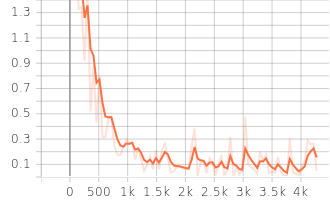
\includegraphics[width=1\linewidth]{../Imgs/train_loss}
\caption{Tensorboard train loss metric}
\label{fig:train_loss}
\end{figure}

\begin{figure}
\centering
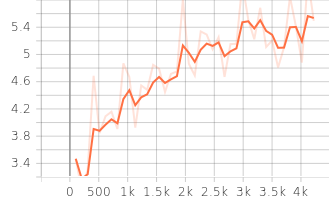
\includegraphics[width=1\linewidth]{../Imgs/val_loss}
\caption{Tensorboard validation loss metric}
\label{fig:val_loss}
\end{figure}

The model overfits even though the following tests have been accomplished:

\begin{itemize}
\item Different number of labels
\item Different stratifications of the train, test and validation set
\item Many different augmentation techniques
\item Different sizes of the Random Crops
\end{itemize} 

All of this was only for training a model on the WikiArt dataset. Apparently, the images in this dataset are not generalizable on a single genre. We can see in Figure \ref{fig:pred} that the model only predicts for one genre. 

\begin{figure}
\centering
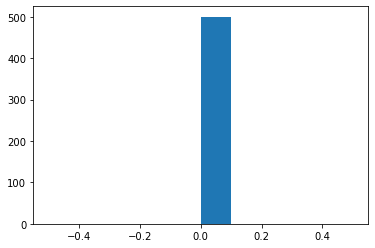
\includegraphics[width=1\linewidth]{../Imgs/prediction_nn}
\caption{Model output after training}
\label{fig:pred}
\end{figure}

\subsection{Clustering on Image Text with LDA}
Focusing on the text of the posters appeared to work significantly better. Although we have no ground truth and therefore cannot compute any metrics about the clustering quality.

We do not know how the LDA clustered the text, but at least we have some examples compared to the classification that did not work. The clusters can be seen in Figure \ref{fig:lda_example}.

\begin{figure}
\centering
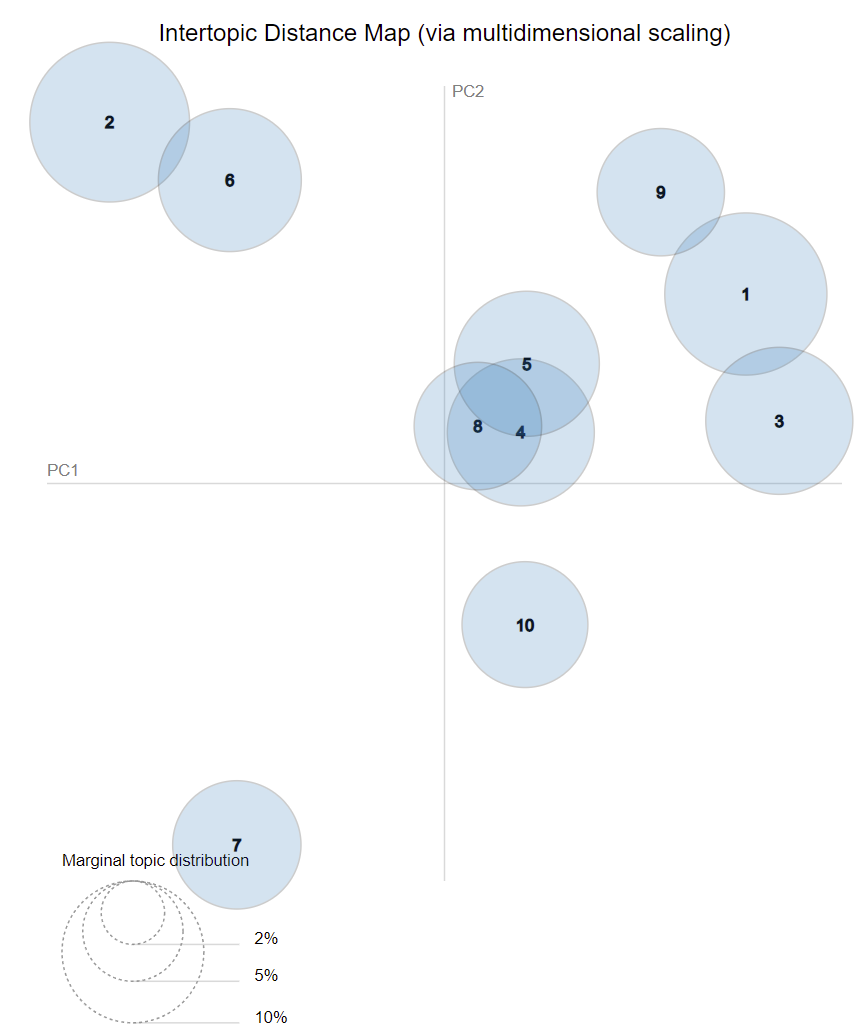
\includegraphics[width=1\linewidth]{../Imgs/lda_map}
\caption{Visualized Clusters of the LDA approach}
\label{fig:lda_example}
\end{figure}

\subsection{Clustering on Image Text with BERT}
The BERT transformer from Google was also implemented into a topic clustering model. This approach appears to be the best working one. After extracting the text from all posters, the most common words are shown in the following Wordcloud in Figure \ref{fig:wordcloud}.

\begin{figure}
\centering
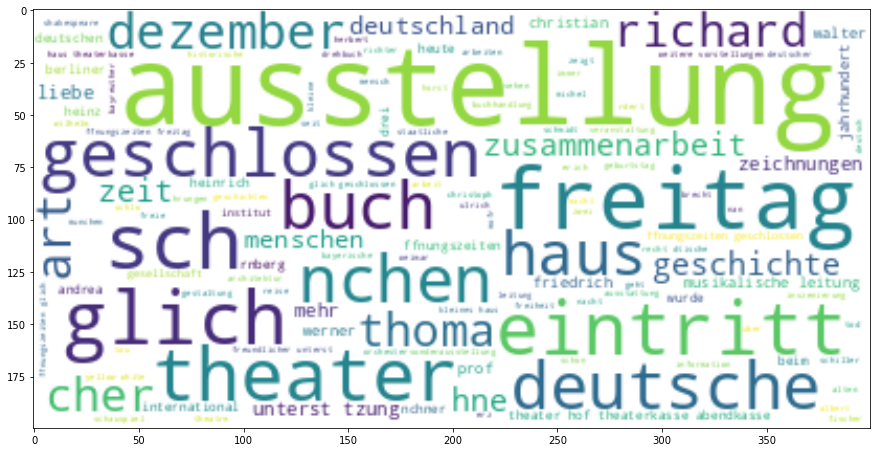
\includegraphics[width=1\linewidth]{../Imgs/wordcloud}
\caption{Wordcloud of the most common words of the poster data}
\label{fig:wordcloud}
\end{figure}

Based on these words, the BERT transformer was applied. In the visualization in Figure \ref{fig:bert_example}, we can see that many clusters were found apart from each other.

A random cluster contains the following words:

\begin{itemize}
\item yellow
\item white
\item theme
\end{itemize} 

Another random cluster contains the following words:

\begin{itemize}
\item Autorenlesung
\item Bibliotheken
\item Improtheater
\end{itemize}

\begin{figure}
\centering
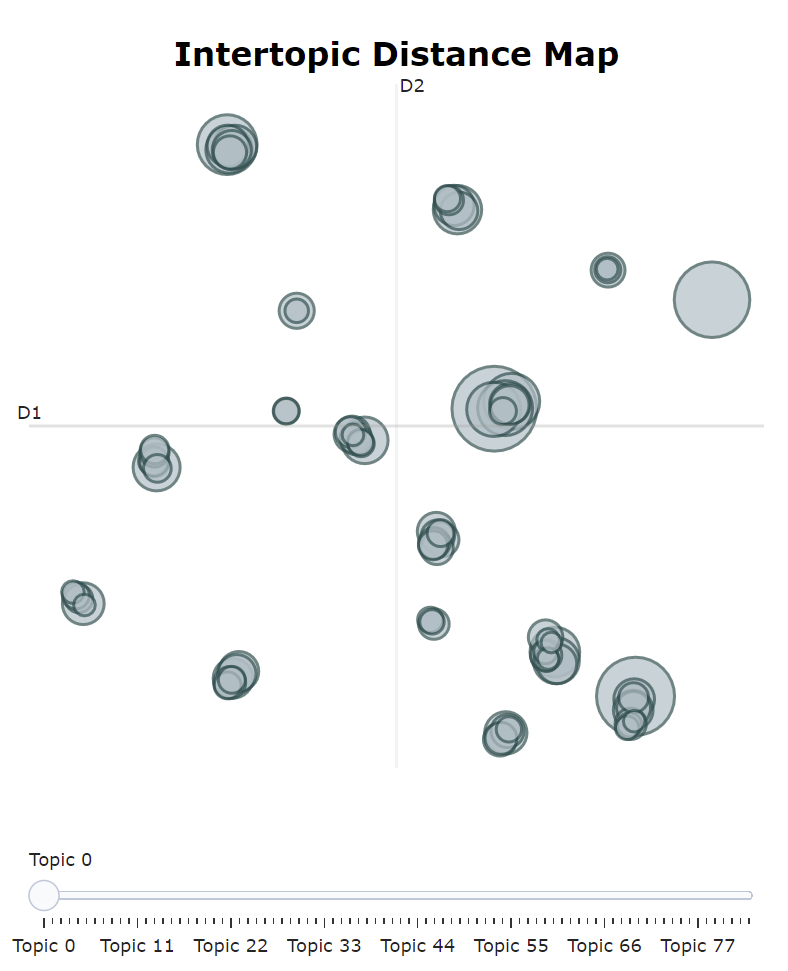
\includegraphics[width=1\linewidth]{../Imgs/bert_map}
\caption{Visualized Clusters of the BERT topic modeling approach}
\label{fig:bert_example}
\end{figure}

We can clearly see connections of the words even without having the same word stem. 

\subsection{Clustering on Image with K-Means}

The unsupervised clustering approach with PCA and K-Means appears to perform second-best among the four approaches. In Figure \ref{fig:kmeans_example} we can detect that the clusters show somehow related images. The text of the images was not used for this approach, only the VGG network to calculate CNN features out of the image. Cluster 3 for example, appears to cluster images with much white content, whereas cluster one clusters complex artworks together.

\begin{figure}
\centering
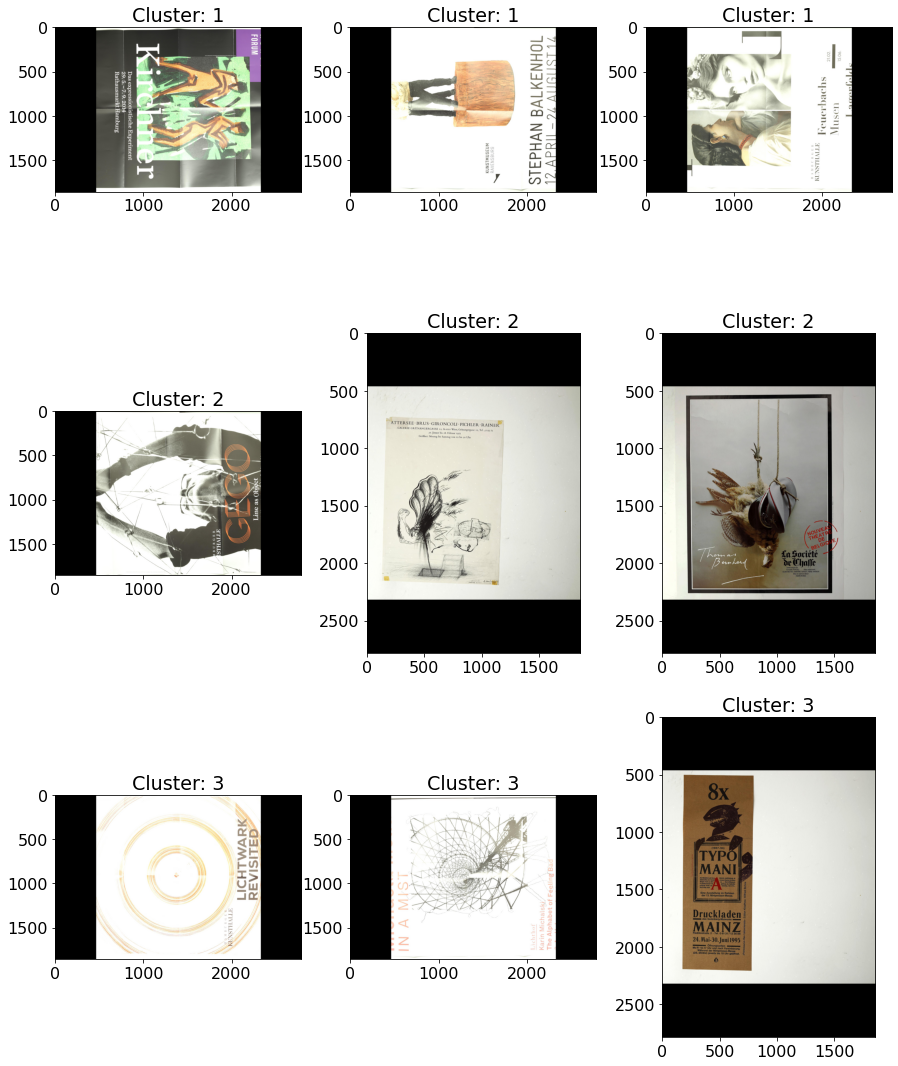
\includegraphics[width=1\linewidth]{../Imgs/image_clustering_example}
\caption{Output of the Image Clustering model for three different clusters with three images each}
\label{fig:kmeans_example}
\end{figure}

The training of this approach is relatively quick, but many steps were required. 

\subsection{Discussion}

None of the methods was satisfying enough to predict effectively the number of clusters or similar posters. The research question can therefore be answered with no, but there exist many more approaches to try. Since we are dealing with poster images, the necessity of the text is not neglectable, but also the use of the image content. Furthermore, since there is no ground truth, at least for the three unsupervised approaches, we need to define metrics or let humans decide if the predicted clusters make sense for some samples. 

\subsection{Future Work}

Many things could be considered to improve current models:

\begin{itemize}
\item Use a better OCR method
\item Try out different parameters like the minimum number of words per poster
\item Use other NLP cleaning techniques for the text
\item Perform Named Entity Recognition (NER) to extent the word list of each poster
\item Impute values if a poster has no words at all
\item Combine Image Clustering and Topic Models
\end{itemize}

I assume that the most impact will have the Named Entity Recognition and the image clustering and topic modeling combination. Since this was a time constraint University IT-Project, I had no more time to investigate these approaches further.

\renewcommand{\refname}{References}
\bibliography{References}


\end{document}
